\documentclass[fleqn,a4paper,12pt]{article}

%used Packages
\usepackage{standalone}		% Zum Einlesen aus anderen .tex-Files
\usepackage{geometry}		% Zur Bearbeitung des Layouts (Ränder,...)
\usepackage[german]{babel}
\usepackage[utf8]{inputenc}
\usepackage{amsmath}		% Mathematische Symbole
\usepackage{amssymb}     	% Nochmehr mathematische Symbole
\usepackage{dsfont}      	% Schriftsatz fuer Zahlenmengensymbole
%\usepackage{verbatim}   	% erweiterte Verbatim-Umgebung
\usepackage{alltt}       	% Quasi-Verbatim-Umgebung
\usepackage{fancyhdr}    	% Eigene Kopfzeilen
\usepackage{graphicx}    	% Zum Einbinden von Grafiken
							% Einbinden einer eps-Grafik geht so: includegraphics{path}
\usepackage{wrapfig}
\usepackage{lscape}
\usepackage{rotating}
\usepackage{epstopdf}

% Skalierung der Grafiken
\setlength{\unitlength}{1cm}

\frenchspacing               % Kein Extrafreiraum nach Satzzeichen
\setlength{\parindent}{0pt}  % Neue Absaetze nicht einruecken
%\sloppy                     % Schlampige Absatzformatierung
\fussy                       % Penible Absatzformatierung
\linespread{1.5}             % Zeilenabstand


% Seitenraender
\geometry{left=30mm, right=40mm, bottom=30mm}
				% Doc-class, Packageimports, fancy stuff
%%Seitenränder formatieren
\addtolength{\voffset}{-2cm}
\addtolength{\textheight}{0cm}
\addtolength{\hoffset}{0cm}
\addtolength{\textwidth}{2cm}
\addtolength{\headheight}{2cm} % fuer jeden Strichkode einen Zentimeter

% Font fuer Code 39
\font\xlix=wlc39 scaled 1200
\newcommand\barcode[1]{{\xlix@#1@}}

% Name, Matrikelnummer, Barcode
\newcommand\student[2]{
	\mbox{\scriptsize
		\begin{tabular}{@{}l@{}r@{}}
			\multicolumn{2}{@{}r@{}}{\barcode{#2}}\\
			#1&#2\\
		\end{tabular}}}

% Kopfzeile
\pagestyle{fancy}            % Eigene Kopfzeilen verwenden
\lhead{
	\small
	\textsc{Grundlagen der Signalverarbeitung \\
		WS 2017/2018 \\
		\"Ubung (\today)}
	\vfill}
\rhead{
	\begin{tabular}[b]{@{}rr@{}}
		\student{Philipp Badenhoop}{572693} &
		\student{Steven Lange}{568733} \\
		\student{Pascal Jochmann}{575056} &
		\student{Kevin Trogant}{572451}
\end{tabular}}			% Definition der Kopfzeile
%andere Definitionen
\providecommand{\R}{{\mathbb R}}
\providecommand{\N}{{\mathbb N}}
\providecommand{\Z}{{\mathbb Z}}
\providecommand{\Q}{{\mathbb Q}}
\providecommand{\C}{{\mathbb C}}
\providecommand{\F}{\mathcal{F}}
\providecommand{\less}{\setminus}
\providecommand{\inv}{{}^{-1}}
\providecommand{\Land}{\bigwedge}
\providecommand{\Lor}{\bigvee}			% Liste der zusätzlichen Commands und redefines

\begin{document}
    \section*{Übungsaufgabe 14}
    Die gegeben Messwerte (N=3):\\
    \begin{tabular}{|c| c| c|}
    	\hline
		\textbf{n}	&	\textbf{$t_n$}	&	\textbf{$f_n$}\\
		\hline
		0	&	-2	&	2\\
		1	&	0	&	1\\
		2	&	1	&	0\\
		\hline
    \end{tabular}\\
	\begin{itemize}
		\item[a.] Annäherung an die Messwerte mit den Basisfunktionen $t^0,t^1$ und $t^2$ durch das Polynom $f_{app}(t) = c_2t^2 + c_1t^1 + c_0t^0$.
		\begin{align*}
			\left(\begin{matrix}f(t_0) \\ f(t_1) \\ f(t_2) \end{matrix}\right)
			= \left(\begin{matrix} t_0^2 & t_0^1 & t_0^0\\t_1^2 & t_1^1 & t_1^0\\t_2^2 & t_2^1 & t_2^0\end{matrix}\right)\cdot\left(\begin{matrix}c_2\\c_1\\c_0\end{matrix}\right)
			= \left(\begin{matrix} 4 & -2 & 1\\0 & 0 & 1\\ 1 & 1 & 1\end{matrix}\right)\cdot\left(\begin{matrix}c_2\\c_1\\c_0\end{matrix}\right) = \left(\begin{matrix}2 \\ 1 \\ 0 \end{matrix}\right)
		\end{align*}
		Nach dem Gauß-Algorithmus ergibt sich dann:
		\begin{align*}
			\left(\left.\begin{matrix} 4 & -2 & 1\\0 & 0 & 1\\ 1 & 1 & 1\end{matrix}\ \ \right|\ \begin{matrix}2 \\ 1 \\ 0 \end{matrix}\right)
			\sim> \left(\left.\begin{matrix} 4 & -2 & 0\\0 & 0 & 1\\ 1 & 1 & 0\end{matrix}\ \ \right|\ \begin{matrix}1 \\ 1 \\ -1 \end{matrix}\right)
			\sim> \left(\left.\begin{matrix} 1 & 0 & 0\\0 & 0 & 1\\ 0 & 1 & 0\end{matrix}\ \ \right|\ \begin{matrix}-\frac{1}{6} \\ 1 \\ -\frac{5}{6} \end{matrix}\right)
		\end{align*}
		Mit diesen $c_i$ gilt:
		\begin{align*}
			f_{app}(t) = B_{M3}(t)	&= -\frac{1}{6}t^2 -\frac{5}{6}t^1 +1\\
			e_{B_{M3}}^2			&= \sum_{i=0}^2\left( f_i - B_{M3}(t_i) \right)= 0
		\end{align*}
		\item[b.] Es sollen die Messwerte mit dem Polynom $f_{app}(t) = c_0t^0 +c_1t^1$ angenährt werden. Nach VL und Buch ist folgende Formel gültig:
		\begin{align*}
			\sum_{n=0}^2\sum_{m=0}^1c_m t_n^mt_n^k = \sum_{n=0}^2f(t_n)t_n^k
		\end{align*}
		Daraus lässt sich folgende Matrix ableiten:
		\begin{align*}
			\left(\begin{matrix}
				\sum_{n=0}^2 t_n^0t_n^0 & \sum_{n=0}^2 t_n^0t_n^1\\
				\sum_{n=0}^2 t_n^1t_n^0 & \sum_{n=0}^2 t_n^1t_n^1
			\end{matrix}\right)\cdot\left(\begin{matrix} c_0\\ c_1\end{matrix}\right)
			=
			\left(\begin{matrix}
				\sum_{n=0}^{2}f(t_n)t_n^0\\
				\sum_{n=0}^2f(t_n)t_n^1
			\end{matrix}\right)
		\end{align*}
		Mit den gegebenen Werte ergibt sich folgende erweiterte Koeffizientenmatrix:
		\begin{align*}
			\left(\left. \begin{matrix}
				3	&	-1 \\ -1 	& 5\end{matrix}\ \ \right|\ \begin{matrix} 3\\-4
			\end{matrix}\right)
			\sim>
			\left(\left. \begin{matrix}
				1	&	0 \\ 0 	& 1\end{matrix}\ \ \right|\ \begin{matrix} \frac{11}{14}\\\frac{-9}{14}
			\end{matrix}\right)\quad\quad\text{nach Gauß-Verfahren}
		\end{align*}
		\begin{align*}
			f_{app}(t) = B_{M2}(t)	=& \frac{11}{14}-\frac{9}{14}t\\
			e_{B_{M2}}^2			=& \sum_{i=0}^2\left( f_i - B_{M2}(t_i) \right) = -\frac{13}{14}
		\end{align*}
		\item[c.] Es sollen die Messwerte mit dem Polynom $f_{app}(t) = c_0t^0$ angenährt werden. Wie in Aufgabe $b.$ gilt:
		\begin{align*}
			\left(\begin{matrix} \sum_{n=0}^2 t_n^0t_n^0\end{matrix}\right) \cdot \left(\begin{matrix} c_0 \end{matrix}\right) = \left(\begin{matrix} \sum_{n=0}^2f(t_n)t_0\end{matrix}\right)
		\end{align*}
		Mit den gegebenen Werte:
		\begin{align*}
			\left(\begin{matrix} 3\end{matrix}\right) \cdot \left(\begin{matrix} c_0 \end{matrix}\right) = \left(\begin{matrix} 3\end{matrix}\right)
		\end{align*}
		\begin{align*}
			f_{app}(t)		&= B_{M1}(t) = 1\\
			e_{B_{M1}}^2	&= \sum_{i=0}^2\left( f_i - B_{M1}(t_i) \right) = 0
		\end{align*}
		\item[d.] Das Interpolationspolynom nach Lagrange ist wie folgt definiert:
		\begin{align*}
			f_{app}(t) = L(t)	=& \sum_{i=0}^2 f_i\cdot \prod_{\substack{j=0\\i\ne j}}^2\frac{t - t_j}{t_i-t_j}\\
								=& 2\cdot\frac{t-0}{-2-0}\cdot\frac{t-1}{-2-1} + 1\cdot \frac{t+2}{0+2}\cdot\frac{t-1}{0-1} + 0\\
								=& 2\cdot\frac{-t}{2}\cdot\frac{1-t}{3} + \frac{t+2}{2}\cdot3\cdot\frac{1-t}{3}\\
								=& \frac{1-t}{3}\cdot\left(\frac{-2t+3t+6}{2}\right)\\
								=& \frac{t+6-t^2-6t}{6}\\
								=& \frac{-t^2-5t+6}{6}\\
						e_L^2	=& \sum_{i=0}^2\left( f_i - L(t_i) \right)= 0
		\end{align*}


	\end{itemize}
	\begin{figure}
		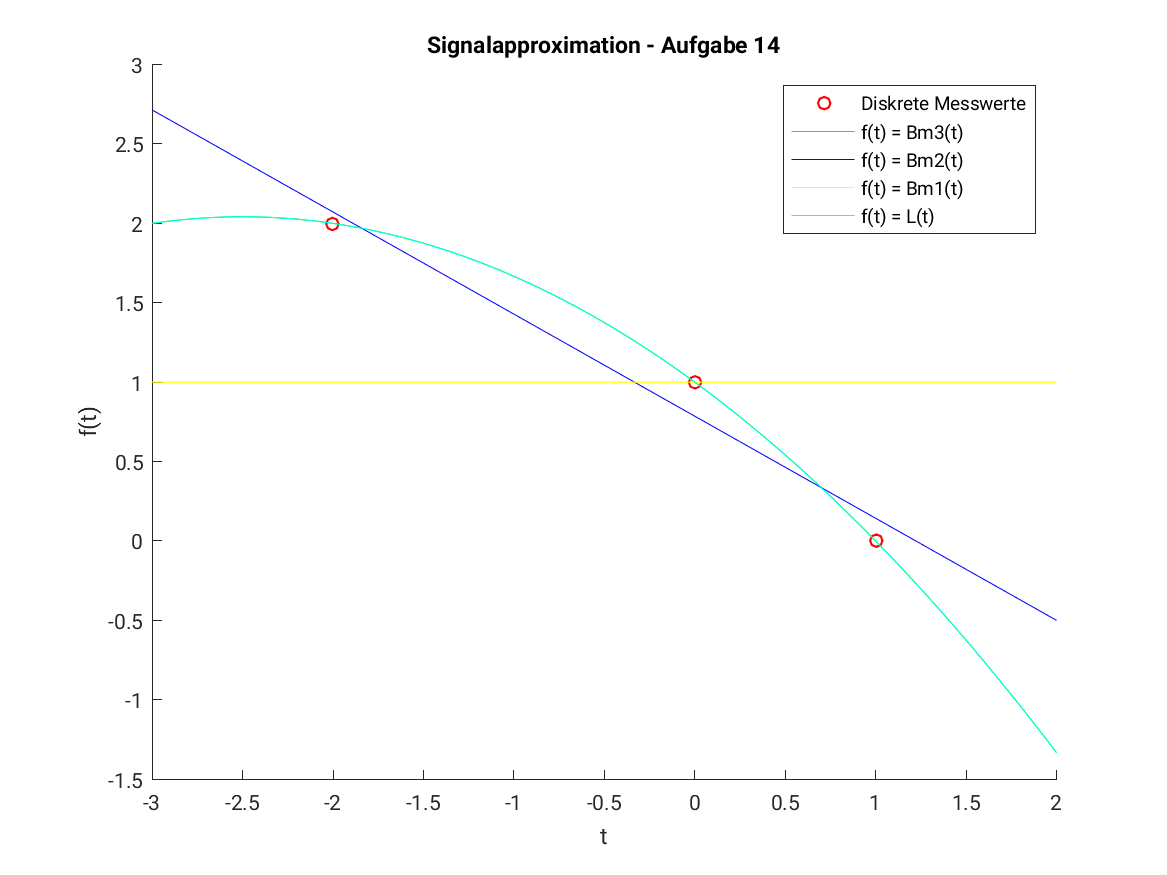
\includegraphics[scale = 0.7]{A14_plot.png}
	\end{figure}
	Es sei zu dem Bild angemerkt, dass $Bm3(t) = L(t)$ gilt.
\end{document}

